\section{PathDS Build and Maintenance}
\label{sec:pds}

In this section, we present a parallelly scalable construction algorithm
for PathDS and an efficient incremental update strategy.



\begin{algorithm}[t!]
  \caption{\kw{PDSBuild}: Parallel PathDS Construction}
  \label{alg:pds-build}
  \SetKwFunction{match}{Match} \SetKwFunction{extend}{Extend}
  \SetKwProg{Fn}{Procedure}{}{}
  \SetKwFunction{match}{Match}
  \SetKwFunction{init}{Init}
  \SetKwFunction{hs}{HSplit}
  \SetKwFunction{ts}{TSplit}
  \SetKwFunction{comp}{Compress}
  \SetKwFunction{getP}{GetsSubPaths}
  \SetKwFunction{maxlen}{MaxLen}
  \SetKwFor{ParaFor}{for each}{do in parallel}{endfor}
  \SetKwFor{ForEach}{for each}{do}{endfor}
  \SetKwComment{KwComment}{\# }{} %%
  \KwIn{Graph $G = (V,E,L)$, a set of path queries $\mathbb{P}$}%%
  \KwOut{PathDS $(\mathcal{S}_s^P, \mathcal{S}_t^P)$ for all $P\in\mathbb{P}$}

  $K \gets \maxlen(\mathbb{P})$; \ \ \
  $\{\mathbb{P}_1, \dots, \mathbb{P}_K\} \gets \getP(\mathbb{P}, K)$; 

  %\ParaFor{$v \in V,\, P \in \mathbb{P}$}{\init{$d_s^P(v), d_t^P(v)$}}
  Initialize $d_s^P(v), d_t^P(v)$ for all $v\in V$ and $P\in\mathbb{P}$;

  \ForEach{$i =1,\dots, K$}{

    \ForEach{$P \in \mathbb{P}_i$}{
      $(s,s', P_1) \gets \hs(P)$; \, \, $(P_2, t', t)\gets \ts(P)$;
      
      \ParaFor{$v\in V$}{
        %  $d_s^P(v) {\gets} \sum\bigl\{ d_{s'}^{P_1}(u)\mid u\in \kw{Nbr}(v),\,\match{v,u,s,s'}\bigr\}$

        % $d_t^P(v) {\gets} \sum\bigl\{ d_{t'}^{P_2}(u)\mid u\in \kw{Nbr}(v),\,\match{u,v,t',t}\bigr\}$
      
        Compute $d_s^P(v)$ and $d_t^P(v)$ via  Eqs.~(\ref{eq:dsP}) \& (\ref{eq:dtP})\;
      \lIf{$P \in \mathbb{P}$}{
        $\operatorname{Update}(\mathcal{S}_s^P, \mathcal{S}_t^P,d_s^P(v),d_t^P(v))$
      } %% IF
      }
    }%% ForEach
  
  }%% ForEach
  
  \Return{$\{(\mathcal{S}_s^P, \mathcal{S}_t^P)\}_{P\in\mathbb{P}}$};
\end{algorithm}

\subsection{Parallel PathDS Construction}\label{susbsec:pds-build}
\eat{
  1、介绍 PDSBuild 的设计原则和核心思想
  - 至底向上构建 flat path degrees
  - 算法并行的粒度，以点为中心进行并行
  2、给出算法1的描述，用文字的描述算法的流程和关键步骤
  3、分析算法的时间和空间复杂度，说明其并行效率和可扩展性
}

We first present \kw{PDSBuild}, a parallel algorithm that constructs
PathDS summaries for a given graph  and a set of path queries .

\vspace{.25em} %%
In a nutshell, \kw{PDSBuild} computes path degrees in bottom-up
manner and updates the corresponding PathDS summaries during the process.
%% 
The algorithm is parallelly scalable in the sense that it guarantees
reduced running time with more processing cores, enabling efficient
PathDS construction on large graphs.



\stitle{Bottom-Up Computation of Path Degrees.} %%
Given a path query $P$, we need the path degrees $(D_s^P, D_t^P)$ to
construct the corresponding PathDS  $(\mathcal{S}_s^P,
\mathcal{S}_t^P)$. %%
A key observation is that $(D_s^P, D_t^P)$ can be derived from the
path degrees of immediate sub-paths, which yields a bottom-up dynamic
construction from shorter paths to longer ones. Let $P=u_0e_1u_1\cdots
e_ku_k$, and define
$\kw{HSplit}(P)=(s,s',P_1)$ and $\kw{TSplit}(P)=(P_2,t',t)$, where
$s=u_0$, $t=u_k$, $s'=u_1$, $t'=u_{k-1}$, $P_1=u_1e_2\cdots e_ku_k$, and
$P_2=u_0e_1\cdots e_{k-1}u_{k-1}$. Then, for each vertex $v\in V$, its
path degrees \wrt $P$ can be computed as follows:
\begin{eqnarray}
  d_s^{P}(v) & = &\sum\bigl\{ d_{s'}^{P_1}(u)\mid u\in
  \kw{Nbr}(v),\,\kw{Match}(v,u,s,s')\bigr\}, \label{eq:dsP}\\
  d_t^{P}(v) & = &\sum\bigl\{ d_{t'}^{P_2}(u)\mid u\in \kw{Nbr}(v),\,\kw{Match}(u,v,t',t)\bigr\}. \label{eq:dtP}
\end{eqnarray}
Here, $\kw{Nbr}(v)$ denotes the set of neighbors of $v$ in $G$, and
$\kw{Match}(v,u,s,s')$ (resp. $\kw{Match}(u,v,t',t)$) checks whether the
data edge is compatible with the corresponding query edge in $P$.
Equations~\eqref{eq:dsP} and \eqref{eq:dtP} therefore reduce the
computation of $(D_s^P, D_t^P)$ to previously computed degrees on $P_1$
and $P_2$. 

\stitle{Parallel Processing.} %%
The path degree computation admits two-level parallelism. We can
process query groups by increasing path length, execute queries within
each group in parallel, and parallelize vertex-wise path degrees for
each query since they are independent given shorter-path results.



\stitle{Algorithm \kw{PDSBuild}}. %%
Putting these together, Algorithm~\ref{alg:pds-build} outlines the
PathDS construction procedure. %
Given a graph $G$ and a set of short path
queries $\mathbb{P}$, \kw{PDSBuild} constructs the corresponding PathDS
summaries $\{(\mathcal{S}_s^P, \mathcal{S}_t^P)\}_{P\in\mathbb{P}}$ for
all $P\in\mathbb{P}$ in parallel. 

\sstab (1) \kw{PDSBuild} first generates all sub-paths of queries in
$\mathbb{P}$ and groups them by length into
$\mathbb{P}_1,\dots,\mathbb{P}_K$ (line~1). %
It then initializes $d_s^P(v)$ and
$d_t^P(v)$ for all $v\in V$ and $P\in\mathbb{P}$ (line~2).

\sstab (2) \kw{PDSBuild} next computes the path degrees in a
bottom-up manner and in parallel (lines~4--7). For each
$P\in\mathbb{P}_i$, it applies $\kw{HSplit}/\kw{TSplit}$ to obtain the
sub-paths of $P$ and, in parallel over each vertex $v\in V$, computes
 $d_s^P(v),d_t^P(v)$ using  Eqs.~\eqref{eq:dsP}--\eqref{eq:dtP}. 

\sstab (3) When $P\in\mathbb{P}$, the computed degrees are mapped to
their ranks and used to update the corresponding rank buckets in the
PathDS summaries defined in Definition~\ref{def:pathds} (line~8).
It the end, \kw{PDSBuild} returns
$\{(\mathcal{S}_s^P,\mathcal{S}_t^P)\}_{P\in\mathbb{P}}$ (line~9).

\stitle{Analysis}. \todo{analyze the time and space complexity of \kw{PDSBuild}}

\subsection{Incremental PathDS Maintenance}\label{susbsec:pds-maintenance}

\plan{
1. 给出增量更新算法的问题定义
2. 介绍增量更新算法的挑战： pathDS 难以直接更新 
  --> 观察： 中间结果 path degrees 是可以增量更新 
  --> 基于观察给出基础方法：
      - 离线存储 path degrees DS, 基于 G, \delta G, 计算 \delta DS 
      - 给出代代码描述流程，参考 Sec 6.1
      - 分析算法的时间复杂度，说明其效率和适用场景
3. 指出基础方法的不足：需要存储全量 path degrees; 且更新效率受 path length 和 graph size 影响
4. 提出优化方法，说明优化方法的性能
}
\newpage

\label{subsec:flatr} a path pattern $P$, FlatDS records the exact number of matches of
$P$ originating from each valid start vertex.
Conceptually, FlatDS corresponds to the most fine-grained statistic
that PathDS can maintain and serves as the reference point for
subsequent compression.

\stitle{Collection Strategy.} [To be filled: description of how FlatDS is collected efficiently for each path pattern $P$, including traversal strategy ...etc].


\subsection{CompressedDS: Design and Representation}
\label{subsec:compress}

While FlatDS provides exact path statistics, it requires storing one
count per start vertex.
For large graphs or multiple path patterns, this results in substantial
space overhead, making it impractical as a maintained summary.

A natural compression strategy is to construct a compact summary
of FlatDS based on its ordered or aggregated distribution.
Such approaches derive their representation from the globally
arranged sequence of counts and often rely on cumulative
relationships among values.

While this can produce concise summaries, the resulting structure
exhibits cumulative dependencies: the representation of one position
is influenced by other values in the ordered sequence.
Consequently, a local modification may affect more than the modified
count itself, potentially requiring adjustments beyond the changed
value.

CompressedDS adopts a different design principle.
Instead of aggregating multiple entries into a shared statistic,
it compresses each FlatDS entry independently.


\stitle{Compression Procedure.} CompressedDS is constructed by applying entry-wise upper-bound compression to FlatDS.
For each exact count $x$, the compression produces a compact descriptor
$(\pi, k)$, where $k = \lceil \log_b x \rceil$ denotes the logarithmic
bucket index under base $b$, and $\pi$ stores the top-$n$ most
significant bits of $x$.
This representation preserves the order of magnitude of each entry
while reducing storage overhead.

For each bucket $k$, we also record the maximum exact value
$M_k$ among all path counts assigned to that bucket.
During cardinality estimation, all values mapped to bucket $k$
are conservatively approximated by $M_k$.

\begin{algorithm}[t]
\caption{FastCompress: Constructing CompressedDS}
\label{alg:fastcompress}
\KwIn{FlatDS $f_P = [x_1, x_2, \ldots, x_m]$, bucket base $b$, prefix length $n$}
\KwOut{CompressedDS $H$ and bucket maxima $\{M_k\}$}

\ForEach{$x \in f_P$}{
  $k \leftarrow \lceil \log_b x \rceil$\;
  $\pi \leftarrow$ top-$n$ most significant bits of $x$\;
  Insert $(\pi, k)$ into $H$\;
  $M_k \leftarrow \max(M_k, x)$\;
}
\Return{$H$ and $\{M_k\}$}
\end{algorithm}

Algorithm~\ref{alg:fastcompress} presents the construction procedure.
Because the algorithm scans FlatDS once and processes each entry independently,
FastCompress runs in linear time in $|f_P|$ and supports streaming
and parallel execution.
Its cost is insensitive to the global distribution of path counts,
and no cross-entry aggregation is required.


\begin{figure}[t]
  \centering
  % Placeholder for CompressedDS layout illustration
  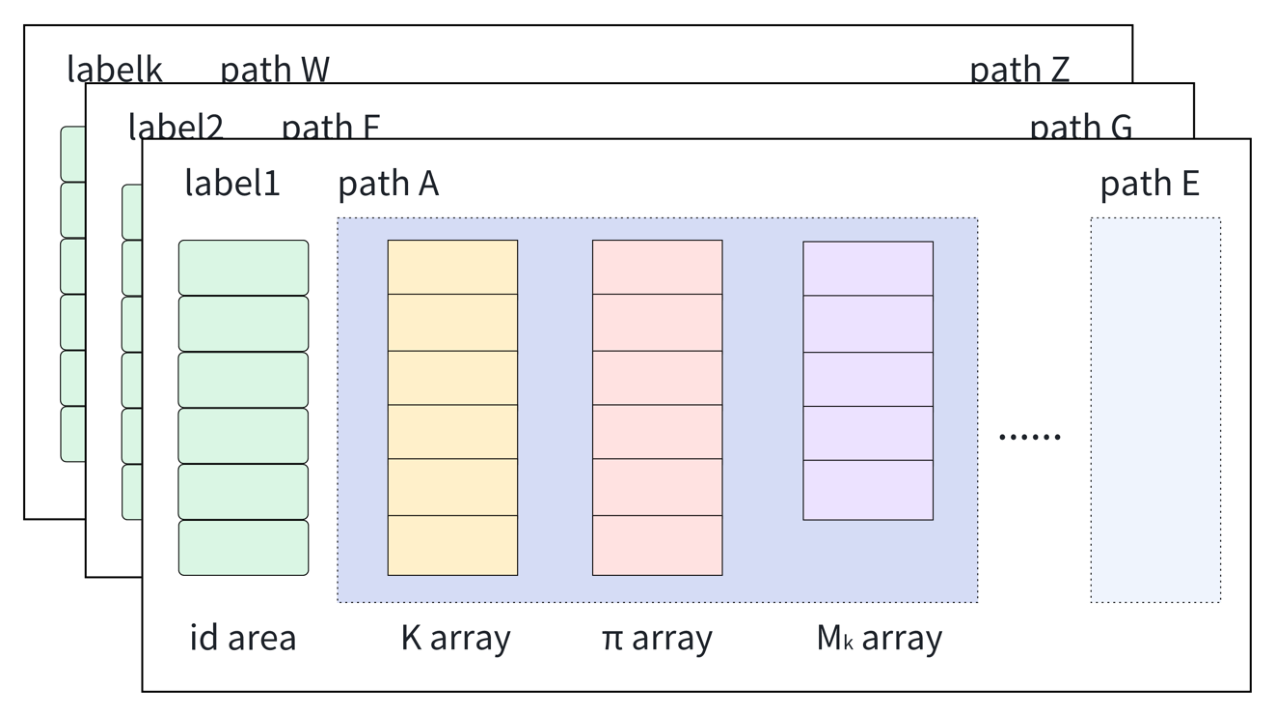
\includegraphics[width=\columnwidth]{figures/sec-pds/CompressedDS_memory_layout.pdf}
  % \fbox{\parbox{0.8\linewidth}{\centering
  % CompressedDS memory layout illustration}}
  \caption{In-memory representation of CompressedDS.}
  \label{fig:compressed_layout}
\end{figure}

\stitle{Memory Layout.} [To be filled:
CompressedDS is stored as a contiguous array of fixed-size entries
representing $(\pi, k)$ pairs.
Bucket-level maxima $\{M_k\}$ are stored in a separate compact array,
indexed by bucket identifier.
This separation allows efficient access to both per-entry information
and bucket metadata while maintaining cache-friendly memory access
patterns.]

\subsection{Incremental Updates}
\label{subsec:update}

With CompressedDS, path count changes can be handled incrementally.
Since compression is independent across path counts, an update
affects only the associated descriptor and its bucket metadata,
without requiring global reconstruction.

When the exact count of a path instance changes by a small value
$\Delta$, the corresponding compressed entry $(\pi, k)$ is updated as
follows.
First, we recover an estimate of the original
value using the current bucket maximum $M_k$.
Specifically, the value is restored as $x = M_k$.
After applying the update, the new value $x' = x + \Delta$ is mapped to a
possibly new bucket $k' = \lceil \log_b x' \rceil$, and a new prefix
$\pi'$ is extracted accordingly.

If $k' = k$, the update does not change the order of magnitude of the
value, and no bucket migration is required.
Only the bucket maximum $M_k$ is updated if $x'$ exceeds the current
maximum.
If $k' \neq k$, the entry migrates to the new bucket $k'$, and both
$M_k$ and $M_{k'}$ are updated accordingly.

This update strategy ensures that each modification affects only
constant-sized metadata,
resulting in amortized constant update cost while preserving
the upper-bound guarantee.



\subsection{Upper-Bound Correctness and Estimation Accuracy}
\label{subsec:theory}

\stitle{Upper-Bound Preservation.}
[proof]

\stitle{Estimation Accuracy.}
[proof]

\newpage